% \iffalse meta-comment
%
% Copyright (C) 2013 by Scott Pakin <scott+thrcl@pakin.org>
% -------------------------------------------------------
%
% This file may be distributed and/or modified under the
% conditions of the LaTeX Project Public License, either version 1.3c
% of this license or (at your option) any later version.
% The latest version of this license is in:
%
%    http://www.latex-project.org/lppl.txt
%
% and version 1.3c or later is part of all distributions of LaTeX
% version 2008/05/04 or later.
%
% \fi
%
% \iffalse
%<*driver>
\ProvidesFile{threadcol.dtx}
%</driver>
%<package>\NeedsTeXFormat{LaTeX2e}[1999/12/01]
%<package>\ProvidesPackage{threadcol}
%<*package>
    [2013/01/06 v1.0 Convert columns to PDF article threads]
%</package>
%
%<*driver>
\documentclass{ltxdoc}
\usepackage{threadcol}
\usepackage{graphicx}
\usepackage{hyperref}
\EnableCrossrefs
\CodelineIndex
\RecordChanges
\setthreadname{User documentation}
\begin{document}
  \sloppy
  \DocInput{threadcol.dtx}
  \setthreadname{Developer documentation}
%  \PrintChanges
  \setthreadname{}
  \makeatletter
  \let\orig@index@prologue=\index@prologue
  \def\index@prologue{%
    \phantomsection\addcontentsline{toc}{section}{Index}
    \orig@index@prologue
  }%
  \makeatother
  \PrintIndex
\end{document}
%</driver>
% \fi
%
% \CheckSum{119}
%
% \CharacterTable
%  {Upper-case    \A\B\C\D\E\F\G\H\I\J\K\L\M\N\O\P\Q\R\S\T\U\V\W\X\Y\Z
%   Lower-case    \a\b\c\d\e\f\g\h\i\j\k\l\m\n\o\p\q\r\s\t\u\v\w\x\y\z
%   Digits        \0\1\2\3\4\5\6\7\8\9
%   Exclamation   \!     Double quote  \"     Hash (number) \#
%   Dollar        \$     Percent       \%     Ampersand     \&
%   Acute accent  \'     Left paren    \(     Right paren   \)
%   Asterisk      \*     Plus          \+     Comma         \,
%   Minus         \-     Point         \.     Solidus       \/
%   Colon         \:     Semicolon     \;     Less than     \<
%   Equals        \=     Greater than  \>     Question mark \?
%   Commercial at \@     Left bracket  \[     Backslash     \\
%   Right bracket \]     Circumflex    \^     Underscore    \_
%   Grave accent  \`     Left brace    \{     Vertical bar  \|
%   Right brace   \}     Tilde         \~}
%
%
% \changes{v1.0}{2013/01/06}{Initial version}
%
% \GetFileInfo{threadcol.dtx}
%
% \DoNotIndex{\@empty,\box,\copy,\def,\else,\fi,\gdef,\global}
% \DoNotIndex{\hss,\ifx,\let}
% \DoNotIndex{\MessageBreak,\newcommand,\protect}
% \DoNotIndex{\setbox,\space,\vbox}
%
% ^^A  Define a few helper commands.
% \DeclareRobustCommand{\pkgname}[1]{\mbox{\textsf{#1}}\SortIndex{#1}{\textsf{#1}}}
% \DeclareRobustCommand{\acro}[1]{\textsc{\MakeLowercase{#1}}}
% \DeclareRobustCommand{\menu}[1]{\textit{#1}~$\to$ }
% \DeclareRobustCommand{\menuentry}[1]{\textit{#1}}
% \makeatletter
% \DeclareRobustCommand{\panel}[1]{\textit{#1}}
% \DeclareRobustCommand{\kbd}[1]{\textit{#1}}
% \DeclareRobustCommand{\AAR}{Adobe Acrobat\slash Reader}
%
% ^^A  Specify this document's metadata.
% \title{The \textsf{threadcol} package\thanks{This document
%   corresponds to \textsf{threadcol}~\fileversion, dated \filedate.}}
% \author{Scott Pakin \\ \texttt{scott+thrcl@pakin.org}}
% \hypersetup{^^A
%   pdftitle={The threadcol package},
%   pdfauthor={Scott Pakin},
%   pdfsubject={Organize document columns into PDF "article threads"},
%   pdfkeywords={LaTeX, PDF, article threads, beads, automatic column scrolling}
% }
%
% \maketitle
%
% \section{Introduction}
% \label{sec:introduction}
%
% Consider the following situation: You have a two-column \acro{PDF}
% file that you want to read on your computer (or tablet or whatever).
% Because you have a relatively small screen---and/or less-than-perfect
% eyesight---you zoom in to more easily read the text.  You read the
% first column of the first page, then scroll back to the top of the
% page and over to the right to read the second column, then scroll left
% to read the first column of the second page, then scroll up and over
% to read the second column, and so forth.  With all this distracting
% scrolling, it's easy to lose track of where you were or what you were
% reading.
%
% The \pkgname{threadcol} package helps you avoid this situation for the
% \LaTeX\ documents you create.  It puts every column into a \acro{PDF}
% ``article thread''.  A user can then opt to have his \acro{PDF} reader
% automatically scroll through the document in proper reading order.  In
% \AAR\ this is accomplished simply by clicking any place in the
% document window where the mouse pointer is shown as a hand with an
% arrow in it.  The user can scroll forward by clicking in the document
% window or pressing \kbd{Enter} and backward by shift-clicking or
% pressing \kbd{Shift}+\kbd{Enter}.  See the \AAR\ \menuentry{Help}
% documents for more information.
%
% \AAR\ provide an \Acrobatmenu{ArticleThreads}{Articles navigation
%   panel} that lists all of the document's article threads and lets the
% user jump to a specified thread.  Figure~\ref{fig:articles-ar9} shows
% what the \panel{Articles} panel looks like in Adobe Reader~9 on Linux.
% The panel may have to be displayed explicitly by the user.  This can
% be done by right-clicking on the navigation-panel button list and
% selecting \menuentry{Articles}.  Alternatively, in \AAR~9, one can
% also follow the \menu{View}\menu{Navigation
%   Panels}\menuentry{Articles} menu path or in \AAR~X and~XI the
% \menu{View}\menu{Show/Hide}\menu{Navigation
%   Panels}\menuentry{Articles} menu path.  If \panel{Articles} appears
% as a pop-up, it can be docked simply by dragging the tab to the
% navigation panel.
%
% \begin{figure}[htbp]
%   \centering
%   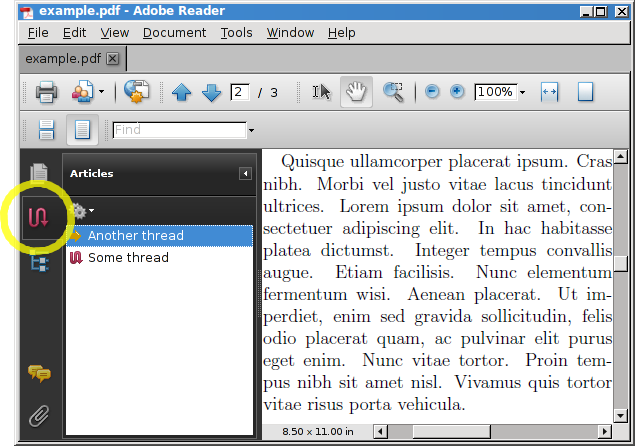
\includegraphics[width=\linewidth]{articles-ar9}
%   \caption{The \panel{Articles} button and navigation panel in Adobe Reader~9}
%   \label{fig:articles-ar9}
% \end{figure}
%
% I don't know if any \acro{PDF} readers other than Adobe's provide
% special viewing of threads.
%
% \bigskip
%
% Although \pkgname{threadcol} is most beneficial to two-column
% documents, it nevertheless also works with single-column
% documents---and even documents that switch between the two using
% |\onecolumn| and |\twocolumn|.  In fact, although it is typeset in a
% single column, this document is itself threaded using
% \pkgname{threadcol}.  Section~\ref{sec:implementation}, which presents
% the commented \pkgname{threadcol} source code, lies in a thread
% entitled, ``Developer documentation''.
% Sections~\ref{sec:introduction}--\ref{sec:limitations}
% and~\ref{sec:future-work} lie in a thread entitled, ``User
% documentation''.  What this structure implies is that you can
% double-click ``User documentation'' in the
% \Acrobatmenu{ArticleThreads}{Articles navigation panel} then
% repeatedly click (or press \kbd{Enter}) on the document's text to read
% all of the user documentation while automatically skipping the
% developer documentation.  Likewise, double-clicking on ``Developer
% documentation'' takes you right to that, bypassing all of the user
% documentation.
%
% Indexes are not normally read from start to finish so this document's
% index is omitted from both the ``User documentation'' and ``Developer
% documentation'' threads.
%
%
% \section{Usage}
% \label{sec:usage}
%
% One of the \pkgname{threadcol} package's goals is simplicity.  All you
% have to do is include a
% \begin{verbatim}
    \usepackage{threadcol}
% \end{verbatim}
% \unskip\noindent
% in your document's preamble for \pkgname{threadcol} to do its work.
%
% \bigskip
%
% \DescribeMacro{\setthreadname}
% One bit of customization that \pkgname{threadcol} does provide,
% however, is control over the name of the article thread.  By default,
% this is ``Entire document''.  However, if you prefer a different name,
% you can write |\setthreadname{|\meta{name}|}| to change the name of
% the article thread to \meta{name}.  It is in fact permissible to
% invoke |\setthreadname| multiple times and with different names.  In
% this case, \pkgname{threadcol} produces one thread per unique name.
% For example, the document shown in Figure~\ref{fig:articles-ar9} used
% two threads in the following manner:
%
% \bigskip
% \begingroup
%   \obeylines
%   |\setthreadname{Some thread}|
%   \meta{Text for the first thread}
%   |\setthreadname{Another thread}|
%   \meta{Text for the second thread}
%   |\setthreadname{Some thread}|
%   \meta{More text for the first thread}
% \endgroup
% \bigskip
%
% \noindent
% When the user clicks on the ``Some thread'' thread, navigation
% automatically bypasses all text in the ``Another thread'' thread and
% vice versa.  One caveat is that in the current version of
% \pkgname{threadcol}, |\setthreadname| issues a |\clearpage| command to
% ensure that text is assigned to the correct thread.  Hence,
% \pkgname{threadcol} cannot currently be used for sophisticated
% magazine- or newspaper-style documents with intertwined threads
% weaving through the pages.  Still, it may be useful for coarsely
% divided units of text.
%
% As a special case, specifying an empty thread name
% (i.e.,~|\setthreadname{}|) stops adding text to threads.  This can be
% useful for a document's front matter and back matter, which may not
% belong in any thread's normal reading order.
%
%
% \section{Limitations}
% \label{sec:limitations}
%
% \pkgname{threadcol} is a fairly simple package.  As such, it has a
% number of limitations, including the following:
%
% \begin{enumerate}
%   \item \pkgname{threadcol} requires pdf\LaTeX\ or Lua\LaTeX; it does
%     nothing when used with ordinary \LaTeX\ or
%     X\lower0.5ex\hbox{\kern-.15em\reflectbox{E}}\kern-0.1667em\LaTeX\@.
%     The package also relies on \pkgname{etoolbox}, which requires
%     \mbox{$\varepsilon$-\TeX} support, but this is provided by all
%     modern \TeX\ distributions.
%
%   \item \pkgname{threadcol} is incompatible with the
%     \pkgname{fixltx2e} and \pkgname{cuted} packages.  These packages
%     redefine \LaTeX's text-output routines in a manner that confuses
%     \pkgname{threadcol}.
%
%   \item Marginal notes (|\marginpar|) are not included in threads.
%     The same is true for text that sticks out into the margin
%     (e.g.,~using |\llap| or |\rlap|), such as the macro names in
%     Section~\ref{sec:implementation}.
%
%   \item As mentioned in Section~\ref{sec:usage}, threads currently
%     must begin on their own page.  Hence, |\setthreadname| forces a
%     page break, which is often undesirable.
%
%   \item \pkgname{threadcol} does not recognize columns created using
%     the |multicols| environment from the \pkgname{multicol} package.
%     These appear to \pkgname{threadcol} as a single column.
%
%   \item No attempt is made to preserve proper reading order beyond
%     page and column order.  For example, if a page ends with the first
%     part of a sentence and the next page begins with a top float, the
%     thread will present the text in that same order: the first part of
%     the sentence, then the float, then the second part of the
%     sentence.  Even worse, \pkgname{threadcol} is oblivious to
%     footnotes that span columns; it will show the first column of
%     text, including the first part of a long footnote, then the second
%     column of text, which ends with the second part of the long
%     footnote.
%
%   \item The package has not been tested thoroughly.  Consequently,
%     there are probably many more limitations than those listed above.
% \end{enumerate}
%
%
% \StopEventually{^^A
%
% \setthreadname{User documentation}
%
% \section{Future work}
% \label{sec:future-work}
%
% A future version of \pkgname{threadcol} may address some of the
% limitations described in Section~\ref{sec:limitations}.  In addition,
% it would great if the package could integrate seamlessly with the
% \pkgname{flowfram} package, where \acro{PDF} article threads would
% make a lot of sense.
%
% One far more difficult change to implement would be to make
% \pkgname{threadcol} cognizant of the ``true'' reading order, perhaps
% with help from the author.  For example, the author could specify the
% point at which the thread should jump to a floating figure before
% jumping back to the corresponding text.
%
% In practice, \LaTeXe's output routines can be quite arcane, especially
% with regards to the handling of inserts (e.g.,~floats and footnotes).
% Getting \pkgname{threadcol} to do more than what it currently does is
% likely beyond my current level of \LaTeX\ expertise.
%
% }
%
% \setthreadname{Developer documentation}
%
% \section{Implementation}
% \label{sec:implementation}
%
% This section is intended for developers and advanced users to learn
% how \pkgname{threadcol} is implemented.  Most readers can ignore this
% section.
%
% \bigskip
%
% We begin by loading a few helper packages upon which we rely:
% \pkgname{ifpdf} to ensure that we have access to |\pdfstartthread| and
% |\pdfendthread| and \pkgname{etoolbox} for the |\patchcmd| macro.
%    \begin{macrocode}
\RequirePackage{ifpdf}
\RequirePackage{etoolbox}
%    \end{macrocode}
%
% \begin{macro}{\thrcl@thread@name}
% Define the name of the current thread.  This is what shows up in the
% \Acrobatmenu{ArticleThreads}{\panel{Articles} navigation panel} in
% Adobe Acrobat and Adobe Reader.
%    \begin{macrocode}
\def\thrcl@thread@name{Entire document}
%    \end{macrocode}
% \end{macro}
%
% \begin{macro}{\setthreadname}
% Let the author change the name of the current thread
% (i.e.,~|\thrcl@thread@name|).  The starred version suppresses the
% |\clearpage|.
%    \begin{macrocode}
\newcommand*{\setthreadname}{%
  \@ifstar{\gdef\thrcl@thread@name}{\clearpage\gdef\thrcl@thread@name}%
}
%    \end{macrocode}
% \end{macro}
%
% \begin{macro}{\thrcl@threaded@box}
% This is a copy of the column box but surrounded by |\pdfstartthread|
% and |\pdfendthread|.
%    \begin{macrocode}
\newbox\thrcl@threaded@box
%    \end{macrocode}
% \end{macro}
%
% \begin{macro}{\thrcl@box}
% Mimic \TeX's |\box| primitive but wrap the given box within a
% |\pdfstartthread| and |\pdfendthread|.  If |\thrcl@thread@name| is
% empty, however, invoke |\box| directly.
%    \begin{macrocode}
\def\thrcl@box#1{%
  \ifx\thrcl@thread@name\@empty
    \box#1
  \else
    \setbox\thrcl@threaded@box=\vbox{%
      \pdfstartthread name {\thrcl@thread@name}%
      \copy#1
      \pdfendthread
    }%
    \box\thrcl@threaded@box
  \fi
}
%    \end{macrocode}
% \end{macro}
%
% \begin{macro}{\thrcl@orig@outputpage}
% We want |\thrcl@outputdblcol| to use the original |\@outputpage| but
% all other invocations to use our modified |\@outputpage|.
%    \begin{macrocode}
\let\thrcl@orig@outputpage=\@outputpage
%    \end{macrocode}
% \end{macro}
%
% \begin{macro}{\thrcl@patchcmd}
% Wrap \pkgname{etoolbox}'s 5-argument |\patchcmd| with a 3-argument
% version that uses hard-wired success and failure operations.  The
% whole command is executed only if all of the previous
% |\thrcl@patchcmd| commands succeeded.
%    \begin{macrocode}
\def\thrcl@patchcmd#1#2#3{%
  \ifx\thrcl@patches@succeeded Y
    \patchcmd{#1}{#2}{#3}{}{\let\thrcl@patches@succeeded=N}%
  \fi
}
%    \end{macrocode}
% \end{macro}
%
% \begin{macro}{\thrcl@outputdblcol}
% \begin{macro}{\thrcl@outputpage}
% \begin{macro}{\thrcl@comdblflelt}
% \begin{macro}{\thrcl@patches@succeeded}
% Replace |\box| with |\thrcl@box| in \LaTeXe's |\@outputdblcol| and
% |\@outputpage| macros, which are used to output a column in,
% respectively, a two-column document or a one-column document.  To
% avoid nesting of |\pdfstartthread|\dots\linebreak[0]|\pdfendthread|,
% we replace calls to |\@outputpage| with calls to
% |\thrcl@orig@outputpage| in |\@outputdblcol|.
%
% Because there we need to apply multiple patches, we attempt to patch
% copies of |\@outputdblcol|, |\@outputpage|, and |\@comdblflelt| and
% replace the originals only if all changes are successful.  We store
% ``|Y|'' in |\thrcl@patches@succeeded| if this is the case,
% otherwise~``|N|''.
%    \begin{macrocode}
\let\thrcl@outputdblcol=\@outputdblcol
\let\thrcl@outputpage=\@outputpage
\let\thrcl@comdblflelt=\@comdblflelt
\let\thrcl@patches@succeeded=Y
\ifpdf
%    \end{macrocode}
% We're in \acro{PDF}-generating mode.  Apply all of our patches.
%    \begin{macrocode}
  \thrcl@patchcmd
    {\thrcl@outputdblcol}%
    {\box\@leftcolumn\hss}%
    {\thrcl@box\@leftcolumn\hss}%
  \thrcl@patchcmd
    {\thrcl@outputdblcol}%
    {\box\@outputbox\hss}%
    {\thrcl@box\@outputbox\hss}%
  \thrcl@patchcmd
    {\thrcl@outputdblcol}%
    {\@outputpage}%
    {\thrcl@orig@outputpage}%
  \thrcl@patchcmd
    {\thrcl@outputdblcol}%
    {\@outputpage}%
    {\thrcl@orig@outputpage}%
  \thrcl@patchcmd
    {\thrcl@outputpage}%
    {\box\@outputbox}%
    {\thrcl@box\@outputbox}%
  \thrcl@patchcmd
    {\thrcl@comdblflelt}%
    {\box}%
    {\thrcl@box}%
  \ifx\thrcl@patches@succeeded Y
%    \end{macrocode}
% All of our patches succeeded.  We can finally redefine
% |\@outputdblcol|, |\@outputpage|, and |\@comdblflelt| for real.
%    \begin{macrocode}
    \global\let\@outputdblcol=\thrcl@outputdblcol
    \global\let\@outputpage=\thrcl@outputpage
    \global\let\@comdblflelt=\thrcl@comdblflelt
  \else
%    \end{macrocode}
% Issue a warning message if any patch failed.  This should happen only
% if a class or package redefines |\@outputdblcol|, |\@outputpage|, or
% |\@comdblflelt| in a manner incompatible with \LaTeXe's default
% definition.
%    \begin{macrocode}
    \PackageError{threadcol}{Failed to patch the output routine}{%
      The threadcol package needs to modify LaTeX's
      \protect\@outputdblcol\space macro to\MessageBreak
      incorporate support for PDF article threads.  These
      modifications failed,\MessageBreak
      presumably due to a class or package that redefined
      \protect\@outputdblcol\space in a\MessageBreak
      form incompatible with what threadcol expects.%
    }%
  \fi
\else
%    \end{macrocode}
% We're not in \acro{PDF}-generating mode.  Warn the author that
% the package will do nothing.
%    \begin{macrocode}
  \PackageWarningNoLine{threadcol}{%
    This package has an effect only when running\MessageBreak
    pdfLaTeX or LuaLaTeX and only when in\MessageBreak
    PDF-generating mode%
  }%
\fi
%    \end{macrocode}
% \end{macro}
% \end{macro}
% \end{macro}
% \end{macro}
%
% \Finale
\endinput
